
\chapter*{FOREWORD}

\begin{figure}
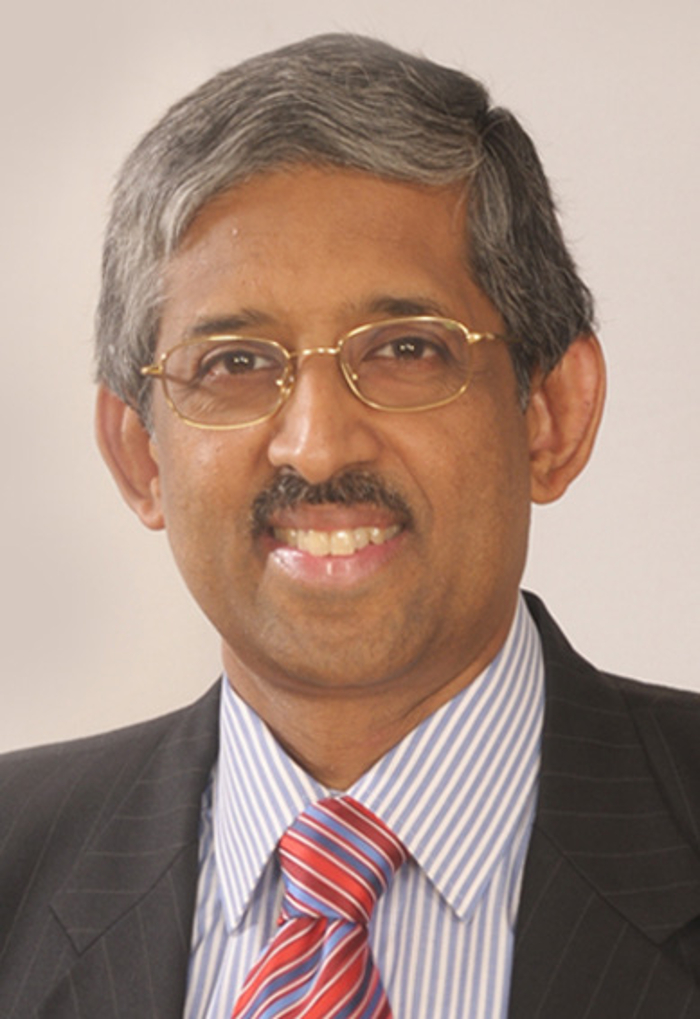
\includegraphics{images/001.jpg}
\caption{\textbf{Padmasri Dr. V. MOHAN,} {\small M.D., FRCP (London, Edinburgh,\\ Glasgow, Ireland), Ph.D., D.Sc., D.Sc (Hon. Causa), FNASc, FASc,\\ FNA, FACP, FACE\\\textbf{President, Research Society for Study of Diabetes in India\\ (RSSDI)\\ Chairman \& Chief of Diabetology, Dr. Mohan’s Diabetes\\ Specialities Centre,\\ Director \& Chief of Diabetes Research, Madras Diabetes\\ Research Foundation,\\ Chennai}}}
\end{figure}

It gives me great pleasure to write this ‘Foreword’ for the book “Diabetes: India's Invisible Enemy” by Dr. V. Lakshminarayan and his son Dr. Sooraj Tejaswi. I have known Dr. Lakshminarayan for many years and admire him for his deep knowledge of Medicine in general, and diabetes, in particular. He is a good speaker, a talented writer, an excellent clinician and above all a great human being. I have always been struck by his humility, his passion for excellence and his deep sense of humility. It is therefore a great pleasure for me to write a Foreword to his book.

Today, diabetes has become a global epidemic and India has the second largest number of people with diabetes in the world, 62.4 million, according to the recent ICMR–INDIAB study results published in 2011. Moreover, it has also an even larger number of people with pre–diabetes (77.4 million). Diabetes is no longer a disease of the rich, the old or urban people. The epidemic is rapidly shifting to younger ages, to rural areas and to the poor. This places a huge burden on not only the individual, family and the society but also the nation, as a whole. A century ago, there was an adage, “Know syphilis and know medicine”. Today, this could be changed to ‘Know diabetes and know medicine’ because diabetes has its ramifications all over the body and produces numerous complications. Moreover it is known as ‘a good disease with bad companions’ because several co–morbidities like hypertension, dyslipidemia, obesity, cardiovascular disease and stroke, non alcoholic fatty liver diseases and even some forms of cancers are associated with diabetes. Therefore the title of Dr. Lakshminarayan’s book “Diabetes: India's Invisible Enemy” is appropriate. A thorough understanding of diabetes, its early detection, prevention and control can help not only individuals with diabetes, but also those with associated diseases and complications. This book covers all aspects of diabetes starting with history of diabetes, the acute and chronic complications of diabetes and various aspects of treatment of the disorder. I congratulate Dr. Lakshminarayan and Dr. Tejaswi on this excellent publication and wish them all the very best with its publication.

\begin{flushright}
\textbf{PADMASRI Dr. V. MOHAN}
\end{flushright}

